% TEMPLATE for Usenix papers, specifically to meet requirements of
%  USENIX '05
% originally a template for producing IEEE-format articles using LaTeX.
%   written by Matthew Ward, CS Department, Worcester Polytechnic Institute.
% adapted by David Beazley for his excellent SWIG paper in Proceedings,
%   Tcl 96
% turned into a smartass generic template by De Clarke, with thanks to
%   both the above pioneers
% use at your own risk.  Complaints to /dev/null.
% make it two column with no page numbering, default is 10 point

% Munged by Fred Douglis <douglis@research.att.com> 10/97 to separate
% the .sty file from the LaTeX source template, so that people can
% more easily include the .sty file into an existing document.  Also
% changed to more closely follow the style guidelines as represented
% by the Word sample file. 

% Note that since 2010, USENIX does not require endnotes. If you want
% foot of page notes, don't include the endnotes package in the 
% usepackage command, below.

\documentclass[letterpaper,twocolumn,10pt]{article}
\usepackage{usenix,epsfig,endnotes, upgreek}
\begin{document}

%don't want date printed
\date{}

%make title bold and 14 pt font (Latex default is non-bold, 16 pt)
\title{\Large \bf Saving pins and power with integrated voltage converters}

\author{
{\rm Michael Barrow}\\
mbarrow@eng.ucsd.edu\\
University of California, San Diego
%\and
%{\rm Second Name}\\
%Second Institution
}

\maketitle

% Use the following at camera-ready time to suppress page numbers.
% Comment it out when you first submit the paper for review.
\thispagestyle{empty}


\subsection*{Abstract}
Recently, demand for increased processor performance coupled with decreasing per-computation power budget has been addressed with emerging parallel processors. Parallel computation is an energy efficient way of increasing performance but requires wider interconnect busses. At the die boundary, the consequence is that systems face an IO bottleneck. The connection between silicon and substrate ends the scope of Moores law in a system, with IO density of packages increasing at a slower rate than on chip.\\
Compounding this problem, addressing performance by increasing paralell units result in increasing energy density due to the end of Dennard scaling. Devices therefore require an increasing number of power pins, further limiting IO pin availability. % ~\cite{Marbell2011}
Integrated power converters are examined in this context. A review of the literature suggests with further research this technique could address the IO bottleneck of future processors.% and power efficiency of future processors.         

\section{Introduction}

%As Moores law continues, Technology scaling gives an increasing number of building blocks to meet conflicting consumer demands of increasing performance and energy efficiency. However the turn right approach exposes architects to complications of inconsistent technology scaling rates. In particular, for IO bound applications, the amount of achievable parallelism in silicon is proportional to the number of IO pins. The  \\

%\begin{itemize}
%\item{\textbf{Motivation}:  crisis has been known for some ti}
%\item{Stakeholders}
%\item{Historical context}
%\item{Current state of art}
%\item{State of art limitations}
%\item{Content of doc}
%\end{itemize}

Against a backdrop of declining PC and growing smartphone sales, mobile devices drive demand for low power, high performance architectures. Emerging applications such as augmented reality, location aware services, high performance games and novel machine interfaces place an increasing demand for expanded IO capabilities and memory bandwidth from generation to generation of these devices. With the number of popular software stacks being lower than the number of major hardware vendors, device battery life is an important product differentiator. Research interest has therefore increased in power efficient architectures that can meet the IO and memory bandwidth requirements of the mobile segment.\\
%DROP THISDespite a drop in PC demand, server 
\indent package IO density is a well known problem to architects. Marbell et al~\cite{Marbell2011} review 130 hardware designs over 30 years and find an unsustainable increase in IO and power pin count, relative to total package pins. Promising solutions have been proposed, with Chang et al~\cite{Chang2010} identifying a subset of practical approaches in 2010. They conclude that voltage scaling as proposed by Dennard et al. ~\cite{Dennard1974} is feasible, but enabled by a sum of techniques in different disciplines.\\
At the architectural level, power converter integration is advised in the worst case, where challenges of sub-threshold leakage prevent further reduction of CMOS voltage and power density prevents further integration of IO intensive system blocks such as memory. Chang's observation is that reducing CMOS voltage has an exponential impact on loss through the power delivery pins. By maintaining pin voltage to devices and reducing operating voltage of CMOS using an efficient on die DC DC voltage converter bridge, an IC has a higher effective power density without increasing the number of power pins.\\
\indent Research into integrated DC DC converters has been an active topic pre-empting Chang for other architectural benefits. Contemporary DC DC converters typically feature bulky passive components. These increase the cost and footprint of mobile systems. Additionally, battery technology does not enjoy the improvement rate of CMOS, so drops of digital operating voltages have opened a gulf between Battery supply voltage and IC input voltages. Techniques for extending battery life such as multiple core voltage domains and the trend of increasing peripheral integration mean CPU's are tending to SOC's and require multiple supply voltages. As an example the 2010 Nvidia Tegra 200 series CPU features 29 voltage rails and requires 29 DC DC converters in the worst case ~\cite{NVidia2010}. %http://www.planetanalog.com/author.asp?section_id=398 http://www.manualslib.com/manual/113617/Nvidia-Tegra-Dg-04927-001_v01.html?page=17
 Against this backdrop, the feasibility of integrated DC DC converters shown by Kurson et al~\cite{Kurson2003} invigorated research interest of integrated DC DC converters. A major motivation is removing the space and component costs of off chip converters (~\cite{PhuckLe2011},~\cite{Hongwei2011},~\cite{Yogesh2010} etc.).\\
\indent State of the art in integrated DC DC converters is exemplified in Intel Haswell CPU's FIVR. Although a comparable in concept DC DC converter exists in the literature~\cite{Sturcken2012}, to the authors knowledge this is the only example of an integrated DC DC converter supplying a CPU at such a power envelope.\\
Intel's literature~\cite{Intel2010} %http://www.psma.com/sites/default/files/uploads/tech-forums-nanotechnology/resources/400a-fully-integrated-silicon-voltage-regulator.pdf
suggests the FVIR is employed primarily to remove components and improve power efficiency. However a comparison of the pinout between Haswell ~\cite{IntelHaswell2014} and the non FIVR predecessor ~\cite{IntelIvyBridge2013} suggests that some power pins were saved too. This is unsurprising as Kurson notes in~\cite{Kurson2003} that power pins could be saved by integrated DC DC converters. Noting that DC DC converters improve the IO density problem, the literature is reviewed to asses the feasibility of optimizing power pins to IO pins by increasing supply voltage of an integrated DC DC converter greatly beyond typical CPU operating voltage.\\
\indent The rest of the document is ordered as follows:\\
\begin{itemize}
\item{Section 2 outlines the operation of the step-down DC DC converter and its critical design parameters}
\item{Section 3 describes the design and associated challenges of integrating DC DC Converters on die}
\item{Section 4 provides summary of recent research in integrated DC DC converters}
\item{Section 5 identifies methods of optimizing IC pin out with integrated DC DC converters and directions for future work}
\item{Section 6 Conclusions of the report}
\end{itemize}
 

%More fascinating text. Features\endnote{Remember to use endnotes, not footnotes!} galore, plethora of promises.\\

\section{Operation of the DC DC converter}

%\textbf{Definition of the problem}\\
DC DC conversion can either increase or decrease input voltage with step-up or step-down topologies respectively. Step-up DC DC converters are beyond the scope of this discussion. Consider a step-up converter outputting a fixed DC power point. In order to maintain this output as the converter input voltage drops, the number of current carrying input pins must increase since $P = IV$ and $P_{Out} = P_{In}\times \eta$, where $\eta$ is converter efficiency.\\
A larger voltage step-up therefore requires a larger number of power pins to maintain $P_{In}$.\\ Packaging constraints have focussed research on reducing power pin count ~\cite{Marbell2011}. As such step-up converters are not discussed.\\
\indent Two popular step-down converters in the literature are presented. A review of the literature highlights critical properties that determine the feasibility of on chip integration.

\subsection{Switched Capacitor step-down converter operating principle}\label{SCOpPrinciple}
%For SC description you can see: https://docs.google.com/a/eng.ucsd.edu/document/d/18fPNSis3hjVwwXtvNOv4B4ni1we3ly9B9yZqkZxr0No/edit
Two types of DC DC step down converter are popular in the literature. Type 1 is the switched capacitor (SC) converter. a simplified canonical $\frac{1}{2}$ series-parallel step-down topology is shown in Figure ~\ref{SCTopology}.\\


\begin{figure}[here]
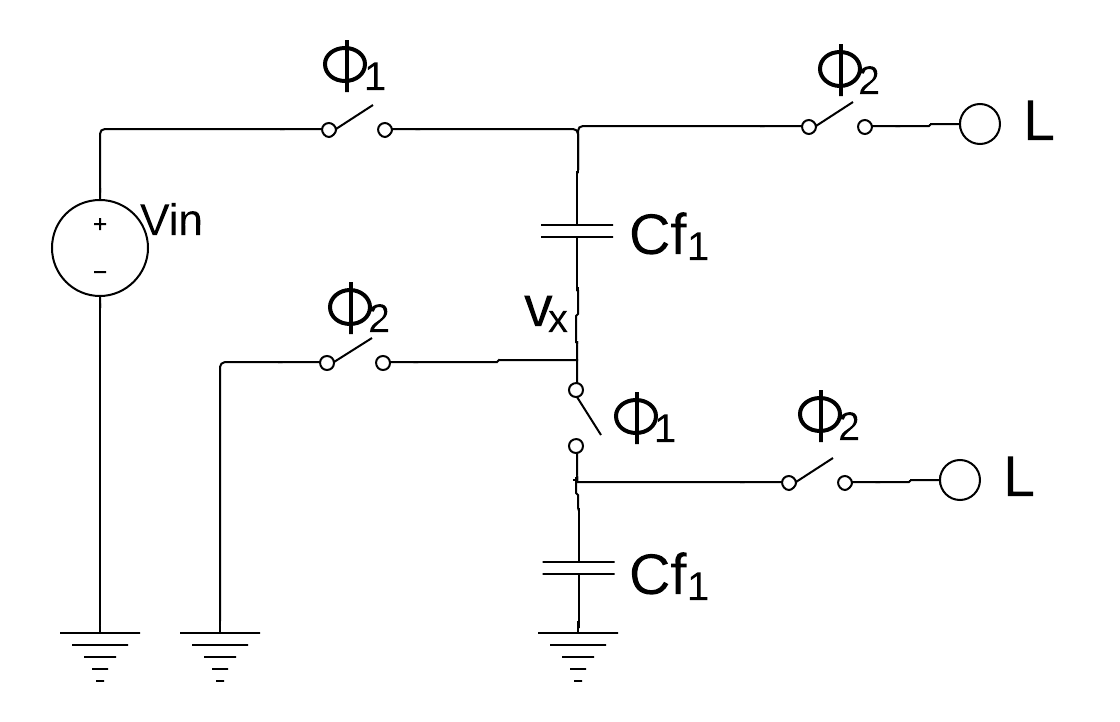
\includegraphics[width=0.4\textwidth]{SCTopology}
\caption{A $\frac{1}{2}$ step-down SC topology with major parasitic components}
\label{SCTopology}
\end{figure}

Let us consider the circuit with ideal components. $Cf$ denotes some capacitance such that $Cf_1 = Cf_2$. switches are controlled by mutually exclusive clocks, $\phi_1$ and $\phi_2$. These clocks are non-overlapping.\\
The circuit has two phases of operation. In phase 1, the charging phase, $\phi_1$ switches are closed and $\phi_2$ switches are open. $Cf_1$ and $Cf_2$ are in series. Since the capacitors are the same size, $V_x$ is $\frac{1}{2}$ of $V_in$.\\
In phase 2, the discharging phase, $\phi_2$ switches are closed and $\phi_1$ switches are open. Now $Cf_1$ and $Cf_2$ are in parallel. Since they are matched in size, $V_x$ remains at $\frac{1}{2}$. Note that the voltage offset of $Cf_1$ moves from $\frac{1}{2} V_{In}$ to $0V$. Therefore, $\frac{1}{2} V_{In}$ is seen at terminal $V_{Out}$ since this is the voltage of both parallel capacitors.\\

\subsection{Inductor-capacitor stepdown converter operating principle}

The second popular converter is the inductor-capacitor step-down (buck) converter. A simplified canonical topology is shown in Figure~\ref{BKTopology}.\\
\begin{figure}[here]
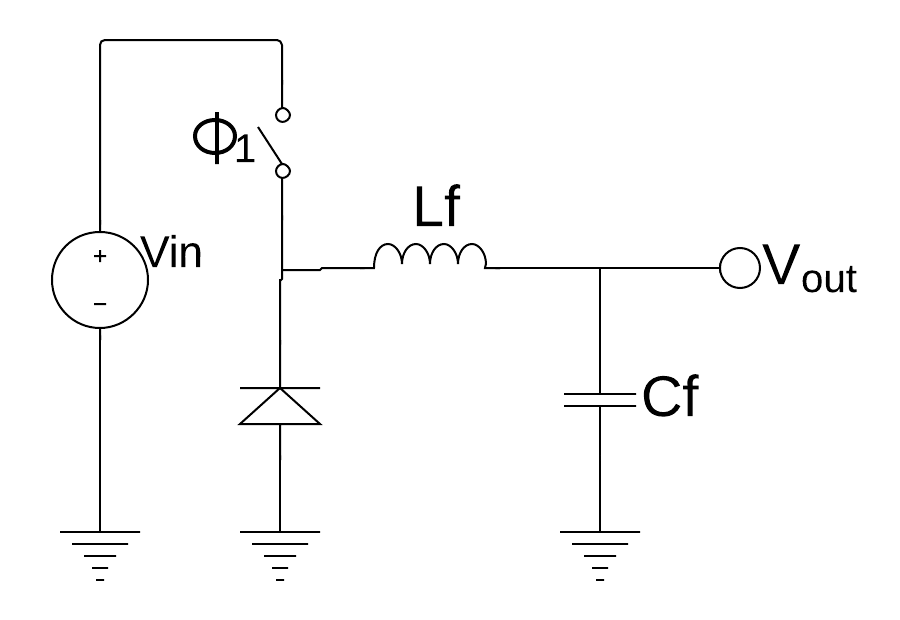
\includegraphics[width=0.4\textwidth]{BKTopology}
\caption{An inductor capacitor buck topology}
\label{BKTopology}
\end{figure}

%For Buck description use chapter 4 of Kurson
The voltage conversion principle is understood by considering the inductor and capacitor as a low pass filter. $\phi_1$ is a clock used to generate a square wave voltage of amplitude $V_{in}$. If this square wave is at a frequency sufficiently higher than the 3db cut-off frequency of the filter, only the DC component of the square wave is observed at $V_{Out}$. Because of this, buck converters may change their voltage step-down ratio during operation, by modulating $\phi_1$. For a converter when current always flows in $L$ (CCM mode), $V_{Out}$ is defined by the duty cycle "$D$"~\cite{Kurson2006} of $\phi_1$ where: $V_{out} = V_{in} \times D$. In other words, if the square wave entering $L_f$ is high for $\frac{2}{3}$ of its period, $V_{out} = \frac{2}{3}\times V_{in}$ and $D = \frac{2}{3}$.\\ 

\subsection{Integrated Converter critical parameters}
If the SC and buck topologies operated without loss, integrated DC DC converters would be trivial to implement, since component size and switching frequencies would be arbitrary. Integrated converters require physically smaller components than substrate mounted DC DC converters. In addition these components can be built with different materials and subject to different loss mechanisms than substrate mounted converters, in order that they are small enough to be integrated in a chip package.\\
The following subsections overview major loss mechanisms of converters and critical parameters that mitigate these losses during converter operation.

\subsubsection{Switched capacitor step-down converter critical parameters}
%Note the \textbf{introduction of $\phi_{\frac{2}{3}}$} This is introduced so when $Cf_2$ has discharged to the load, $Cf_1$ may be connected to restore the supply voltage seen at node $L$. \textbf{we do this because the parasitic resistance of $Cf_1$ and $Cf_2$ is larger in series, maintaining Vout for longer (also fucks with your load impedance, why do it??!!)}\textbf{WE SEE THAT IT IS CRITICAL TO HAVE HIGH FREQUENCY IN ORDER TO MAINTAIN SUPPLY VOLTAGE}


\textbf{Optimum topology: }The energy that a SC converter can transfer per charge cycle is $E_{Isc} = CV^2$. We could therefore express $W = E_{Isc}\times F_\phi$.\\
For a design with a given $V_in$ and ideal components, the designer has two degrees of freedom in designing a converter to power a load, $C$ and $F_\phi$.\\  
We re-draw Figure~\ref{SCTopology} with non-ideal components in Figure~\ref{NonIdealSCTopology}.\\
\begin{figure}[here]
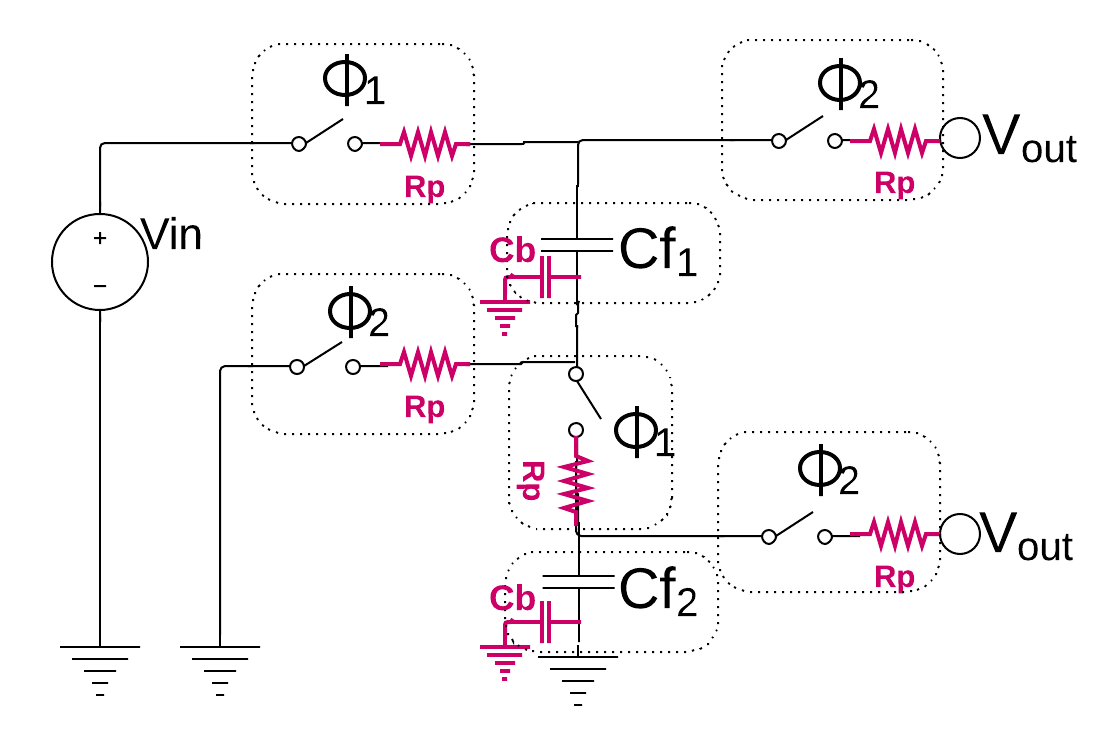
\includegraphics[width=0.4\textwidth]{SCTopologyParasitics}
\caption{An SC topology with major parasitic components}
\label{NonIdealSCTopology}
\end{figure}
\begin{figure}[here]
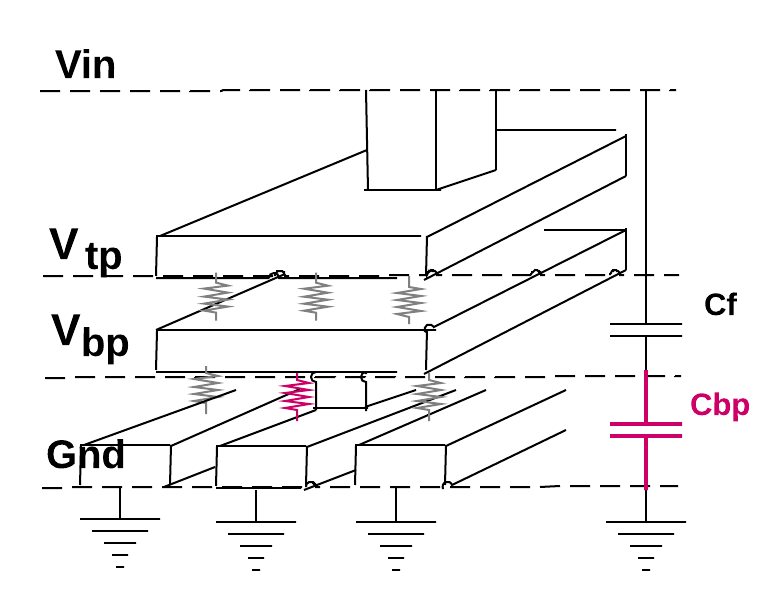
\includegraphics[width=0.4\textwidth]{BottomPlateCap}
\caption{Bottom Plate parasitic capacitance}
\label{BottomPlatePar}
\end{figure}

%The $R_p$ ESR loss of power switches is significant as all power is transferred through switch ESR. The $C_b$ bottom plate capacitance loss is particularly significant with integrated SC because close proximity between the plate and gnd forms large parasitic capacitors from which charge can leak    
By observation of Figure~\ref{NonIdealSCTopology} and Figure~\ref{BottomPlatePar} we see that $F_\phi$ and $C$ are critical parameters that must be optimised to minimize losses.\\
Determining values for $F_\phi$ and $C$ depends on where the dominant loss mechanism is in the converter. An overview of the constituent components and their losses in integrated converters is presented below as primer for evaluating the literature.\\ 
\textbf{Switching losses: }Losses associated with switches are comprised of dynamic loss during the non-overlapping period of $\phi$, and conduction loss due to the equivalent series resistance (ESR) of switches. Dynamic loss is examined in context in Section~\ref{DesignOfIntegratedDCDCConverters}\\
Conduction loss reduces the supply voltage seen at the capacitors by a factor $\delta V_a$. Conduction loss is therefore sensitive to the step-down ratio. Increasing the step-down ratio increases the number of series switches between all capacitors during the charging phase. For example a ratio of $\frac{1}{3}$ has 2 series switches, one of $\frac{1}{4}$ has 3 series switches and so on.\\
\textbf{Capacitor losses: }Losses associated with capacitors are parasitic capacitance losses. A parasitic capacitance known as bottom plate capacitance, depicted in Figure \ref{BottomPlatePar}, exists between one plate of each capacitor and ground. The voltage of these parasitic capacitor is a virtual ground and reduces the supply voltage seen at the capacitors by $\delta V_b$. Their charge can leak to true ground but cannot reach a load. As they are smaller than useful capacitance, they are significantly charged and discharged on each cycle of the converter. Loss is therefore expressed as $W = E_{Pc} \times F_\phi$ where $E_{Pc} = \alpha CV^2$ ~\cite{Damak2013}. Literature reports this to be the second highest loss mechanism in SC converters with bottom plate capacitance up to 5\% of $C_{tot}$~\cite{Ramadass2007}. We also note that $F_\phi$ is adjustable at runtime yet $C$ is not. Parasitic capacitance increases with capacitor area or the size of $C$ and $I_{out} \propto C$~\cite{Damak2013} as well as $F_\phi$. Strategies to reduce bottom plate loss are therefore attractive since they lead to more efficient large capacitors, which in turn reduces the required $F_\phi$. Both effects are desirable since they improve efficiency.\\
%Move load regulation to different sub section SC converters by topology have difficulty 
\textbf{Circuit noise: }SC converters are relatively noisy compared with buck converters because they do not have the built in output filter of the buck. Output noise is therefore strongly related to %bounce of the power switches and 
high inrush current to the power capacitors~\cite{Zheng2013}. As such characterisation of the noise depends on switch and capacitor device parameters, with mitigation achieved through careful switch design and timing control to reduce high frequency noise. 

%In SC converters then, careful design considering voltage specification and technology parameters optimises converters to their load, with noise being addressed via control circuitry. 

\subsubsection{Inductor-capacitor converter critical parameters}

Owing to the similar basic components employed in the buck converter, critical parameters are first identified by differentiating the circuits at the component level. Next, inductor losses are briefly reviewed. Finally, buck transient behaviour is more complex than SC. A brief overview of power and noise in the circuit is therefore provided as an aid to understanding trade-off for the critical circuit parameters.\\
Figure~\ref{BKTopology} represents Figure~\ref{NonIdealBuckTopology} with major parasitics.\\
\begin{figure}[here]
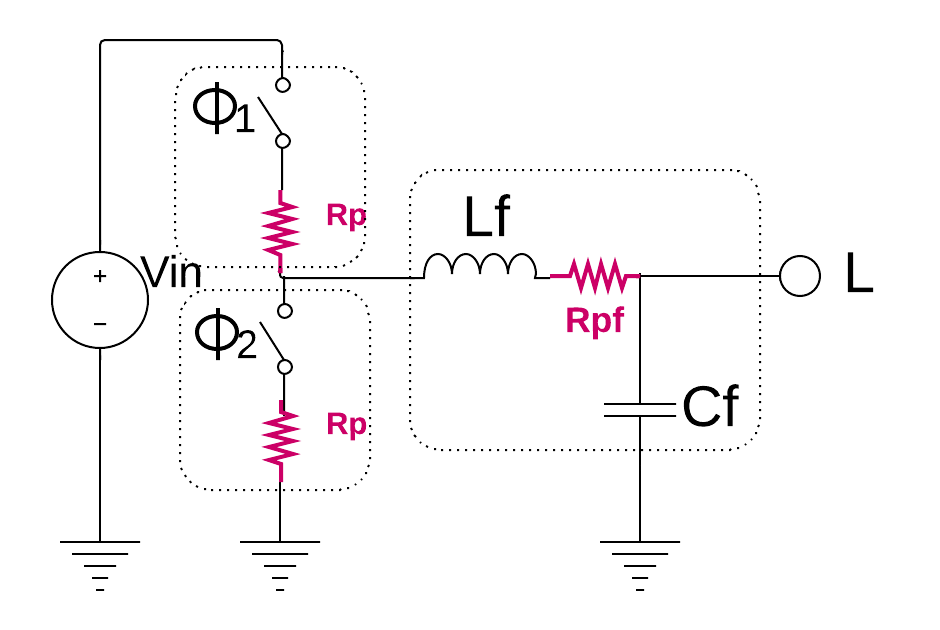
\includegraphics[width=0.4\textwidth]{BuckTopologyParasitics}
\caption{A buck topology with major parasitic components}
\label{NonIdealBuckTopology}
\end{figure}
An extra MOSFET switch is common in the literature and replaces the diode of Figure~\ref{BKTopology}. $\phi_1$ and $\phi_2$ are mutually exclusive and when $\phi_2$ is closed, a clockwise current loop is induced by the charged inductor, as occurs in the diode circuit of Figure \ref{BKTopology}. Introducing this device gives buck and SC converters a common power switch loss mechanism at each phase of operation, but the basic buck features fewer switches contributing to losses than even the most basic SC.\\
\textbf{Inductor Losses: }We now consider the inductor parasitics, given all other power train components are common with SC converters.\\
Losses associated with the inductor are dominated by equivalent series resistance (ESR). Standard CMOS only permits for planar inductors. Increasing inductance is accomplished with a spiral coil to increase flux linkage High inductance requires high numbers of coils per unit area, which translates to increased series resistance (ESR) through the coil.\\
Besides the ESR, the series connection with capacitor $C$ introduces impedance $Z_{LC}$ determined by the $F_{Sw}$ of the buck. It is critical to match $L$ to $F_{Sw}$ and $C$ to minimise this impedance, but the ESR may never be removed.\\  
\textbf{Circuit noise: }With the voltage step-down principle understood we consider the circuit in Figure \ref{BKTopology} from a current perspective. We cannot directly apply Kirchoffs law due the AC variation of $I$ with $T$. However $P_{In} = P_{Out}$ for conservation of energy. Power can only enter the system when current flows through the closed switch from $V_{In}$. Due to either the diode in Figure~\ref{BKTopology} or open circuit switch in Figure~\ref{NonIdealBuckTopology}, its path to the load must be through the inductor. Inductors impede current less as they are charged, therefore for some $T_{On}$ a high $P$ system can be realized if either;\\
\begin{enumerate}
\item{\textbf{$L$ is small relative to $T_{On}$}: A very small inductor is charged significantly over a short time}
\item{\textbf{$T_{On}$ is large relative to $L$}: A large inductor is charged for a very long time}
\end{enumerate}

We consider that during $T_{Off}$, the inductors charge dissipates through the rest of the circuit as current driving the load and parasitic components. Let $T = T_{On}+T_{Off}$ and $F_{Sw} = \frac{1}{T}$ so now 1 and 2 correspond to designing a buck with either;\\
\begin{itemize} %\addtocounter{enumi}{2}
\item{A high $F_{Sw}$ and small $L$ for scenario 1}
\item{A low $F_{Sw}$ and high $L$ for scenario 2}
\end{itemize}
Since the voltage step-down principle is understood, it follows that the choice of $L$ determines the choice of $C$ to minimise $Z_{Out}$ for the desired DC operating points of $V_{Out}$ with a given fixed $F_{Sw}$.\\
Another intuitive observation is that lower $P$ requirements result in $L$ and $F_{Sw}$ values that are easier to realise for given technology limitations, since $P \propto L\times F_{Sw}$. More precisely $P = V_{Out}\times \frac{V_{In}(1 - D)}{2L}DT$ for the maximum load condition.\\ %http://en.wikipedia.org/wiki/Buck_converter#Theory_of_operation
\indent As is common in analogue circuit design, transient operating points complicate the choice of components. A brief overview of solutions provides context for evaluating component loss and trade-off.\\ % Buck converters have dominated medium to high power converter designs for many years~\cite{Sanders2010} and design "rules of thumb" exist in the literature to guide component choice based on required performance.\\
A given digital circuit load has operating conditions that must be satisfied. The following parameters are used to design operating point behaviour for a buck: % input to the buck "rules of thumb"\\
\begin{itemize}
\item {\textbf{Current ripple, $\Updelta i_{Out}$: }Tolerable current variation through the load}
\item {\textbf{Voltage ripple, $\Updelta v_{Out}$: }Tolerable supply voltage noise at the load}
\item {\textbf{Switching frequency $F_{Sw}$: }Nominal switching frequency of the power switches, lower reduces power loss but increases $\Updelta v$ and $\Updelta i$}
\item {\textbf{Operating voltages $V_{In}$,$V_{Out}$: }Nominal input and output voltage of the converter}
\item {\textbf{Maximum drive power $P$: }Converter Power at the highest DC load. $P = V_{Out}\times I_{Max}$} 
\end{itemize}   

$\Updelta i$,$\Updelta v$,$V_{Out}$ and $P$ are constraints specified by the load.\\
$V_{In}$,$F_{Sw}$ along with the passive components $C$ and $L$ must be chosen to satisfy the load constraints as well as technology constraints.\\
\textbf{$\Updelta_i$ Current ripple: }Digital circuits require low supply ripple for deterministic operation. Supply current ripple is defined as\\
$\Updelta i_{Out} = \frac{(V_{In} - V_{Out})D}{2LF_{Sw}}$ ~\cite{Kurson2006}\\
The current flow principle of the buck is understood, so it follows that this formulae does not involve $C$\\
\textbf{$\Updelta_v$ Voltage ripple: }Digital circuits require low voltage ripple for reliable operation. Typically $\frac{V_{Load}}{10}$ is specified. Supply voltage ripple is defined as\\
$\Updelta v_{Out} = \frac{(V_{In} - V_{Out})D}{16LCF_{Sw}^2}$ ~\cite{Kurson2006}\\
The voltage filtering behaviour of the buck is understood, so it follows that this formula involve $F_{Sw}$, $L$ and $C$\\

\indent In summary the loss mechanisms in the buck converters offer more degrees of freedom for optimisation than SC designs because of the additional component type of the inductor. The ripple formulae are useful in limiting aggressiveness applied to any particular parameter and can be used to balance the losses of power train components.

\subsubsection{Converter load regulation concept}
Load regulation is matching output impedance "$Z_O$" of a power converter to a current load. Because $I= \frac{V}{Z_O}$ and maintaining $V$ for a digital circuit is critical, converter output impedance must track quickly with the load condition to keep $V$ constant. The responsibility of tracking load and adjusting $Z_O$ belongs to control circuits. A block diagrams is shown in figure~\ref{ControlCKBlockDiags}\\
\begin{figure}[here]
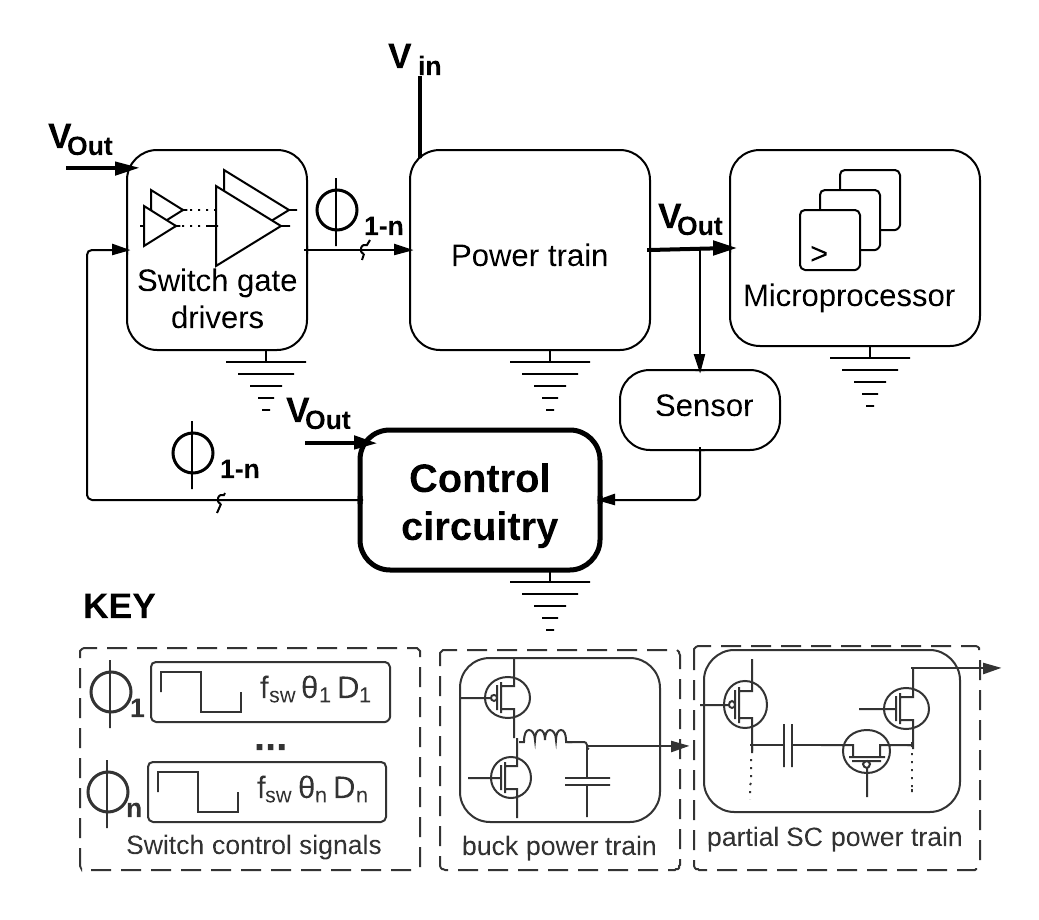
\includegraphics[width=0.4\textwidth]{BasicControlBlockDiag}
\caption{Basic DC DC converter control loop where:
$\theta_x$ = phase, $D_x$ = duty cycle}
\label{ControlCKBlockDiags}
\end{figure}
Buck converters can reduce $Z_O$ by increasing conductance. This is done by increasing "$D$"~\cite{Kurson2006}. Because the asymptote is impedance of the filter at $F_S$, $Z_O$ may also be increased by reducing $F_S$~\cite{Alghamdi2012}.\\ %may want to change ref...
SC converters power loads capacitively. Because the capacitors supply a DC load in parallel, $Z_O$ cannot be lowered below $Z_C$ + $Z_{Sw}$ at the nominal $F_{Sw}$. Modulating $F_{Sw}$ can increase impedance in practice, because the capacitors can be purposely under-charged~\cite{Seeman2008}.\\
%Talk about trade-offs? No I think put that in problems  

\section{Design of Integrated DC DC Converters} \label{DesignOfIntegratedDCDCConverters}

Practical integrated converters are emerging and designed with different goals. A taxonomy of reviewed literature identifies two groupings:\\
\textbf{1: Power system replacement converters}. The research aim is to remove external VRMs with an equal performing integrated subsystem\\
\textbf{2: LDO replacement converters}. The research aim is an incremental improvement of the Low-drop-out (LDO) regulators that have long been integrated on chip.\\
These differing goals result in different design trade-offs We focus on group 1 because of an efficiency reason. To explain, consider the operating principle of an LDO. A transistor gate is biased in its linear conduction region and a fixed voltage is dropped from source to drain to give desired $V_{Out}$. Recall power transfer efficiency, $\eta = \frac{R_{Load}}{R_{Load} + R_{Source}}$. For an LDO, MAX($\eta$) = 0.5. Using a comparable integrated converter to optimize power pins is intractable because around half the power budget is wasted as heat, clearly a sub-optimal design. As such, literature aiming at group 1 best aligns with this reports interest in pin count optimisation.\\  

\subsection{Motivation}
Switching converters such as the SC and buck can offer far higher efficient energy transfer than linear types. Theoretical efficiencies have been modelled at 96\%~\cite{Rodriguez2014} using state of the art devices. Integrated buck and SC implementations have been reported with 84\%~\cite{Cheng2013} and 93\%~\cite{Damak2013} efficiency respectively. Provided these power converters can drive the desired load of a processor, they could be used to obtain an optimum IO to power pin ratio for a processor. This would be accomplished by increasing the input voltage to on die converters to reduce the number of supply pins until a desired number is reached.  

\subsection{Design challenges}
An Integrated DC DC converter is optimized through design trade-offs that consider component non-idealises Given that CPU designs have differing power envelopes and CMOS processes have unique electrical properties, researchers have explored the design space at multiple entry vectors.\\  
\indent \textbf{SC converters} The entry vector is an argument that
\begin{itemize}
\item{Capacitance is easy to implement because MOSFET gate capacitance is a basic building block of CMOS. No corresponding basic block exists for inductance.}
\item{Inductors have a necessarily large parasitic impedance because they are made from coiled resistive wire. Capacitors have a lower minimum impedance which shrinks as the plate size or capacitance grows.}
\end{itemize}
 
However, it has been evidenced this type of converter has less flexible output impedance as compared with buck converters. Also SC converters do not have a voltage regulating filter which is built-in to bucks. This makes their output voltage vulnerable to switching noise.\\
Therefore the design challenges emphasised in SC converters are maximising effective capacitance, controlling output impedance and regulating output voltage.\\ 
%\textbf{Problems of bottom plate parasitic cap}. Bottom plate parasitic capacitance limits the attractiveness of SC designs. \\
%Problems of switching noise. These designs are noisier than Bucks, which have a filter by design\\
\textbf{buck converters} The entry vector is an argument that
\begin{itemize}
\item{Inductors can be implemented in standard CMOS} 
\item{Inductor based buck has been a preferred design for ($>$100mW) applications over the past several decades ~\cite{Sanders2010}, why change this?}
\end{itemize}

Drawbacks of buck converters are noted earlier as arguments in favour of an SC design.

\subsection{Performance drawbacks of Baseline monolithic DC DC Converters}
Early examples of a CMOS integrated SC converter \cite{Viraj2007} and CMOS integrated buck converter \cite{Alimadadi2008} demonstrate the starting point for contemporary integrated converter research. These designs highlight the performance drawbacks of baseline CMOS for integrated converters and deviate from the entry vector arguments supporting each design. As such this literature explains the present concentration of research interest in more recent work. %These setbacks from the initial entry vectors arguments for integrated SC or buck converters also explain the research and design approaches taken in more recent work. 
Although one process generation separates the designs, they are reasonably compared since the power components (capacitors, inductors and switches) consume almost all of the die in both designs.\\ 
\textbf{SC drawbacks: } Naive Integrated SC converters have a low power density. \cite{Viraj2007} realize an on die capacitance of 1600pF with a converter power density of 1.7$mW/mm^2$. In comparison  the baseline buck \cite{Alimadadi2008} realize on die capacitance of 1.1nF with a power density of 20$mW/mm^2$.\\
The baseline SC converter also realizes much lower efficiency than expected Viraj et al. expect. $80\%$ is predicted in the literature, but only $62\%$ is achieved due to un-modelled parasitic losses.\\
Only a single step-down voltage ratio is implemented, since the fixed SC circuit topology described in section \ref{SCOpPrinciple} is used. As such, impedance matching is not possible in this work\\
The performance of this design focussed researchers in areas to make SC integrated converters attractive in replacing off chip IC power converters. Broad categories and related research are listed below.\\
\begin{itemize}
\item \textbf{Energy density: }Device technology research to improve capacitor energy density
\item \textbf{Efficiency: }Technology, circuit topology and converter control research to reduce power leakage
\item \textbf{Flexibility: }Improve load regulation with SC power circuit topology and SC converter control research. In other words, provide flexible step-down ratio's. 
\end{itemize}
\textbf{buck drawbacks} Although power density is higher than the baseline SC, it is still too low for many contemporary processors. \\
Naive Integrated buck converters have a low efficiency. Alimadadi et al. \cite{Alimadadi2008} achieve a peak efficiency of $46\%$. Not only is this lower than the baseline SC \cite{Viraj2007}, its lower than an LDO ($50\%$).\\
Unlike the SC design, the baseline buck can implement a range of step-down voltages in a basic topology. However the baseline has poor load regulation. At its lowest output voltage it has a $25\%$ efficiency in its most sophisticated control mode. This drops to $13\%$ in its baseline mode.\\ 
As with the SC design, the issues in this and other early monolithic converters led researchers to focus on areas of improvement to make integrated buck converters suitable to replace discrete IC's. The broad categories and related research are summarized below.
\begin{itemize}
\item \textbf{Energy density: }Device technology research to improve inductor energy density
\item \textbf{Efficiency: }Technology, buck circuit topology and buck converter control research to reduce power leakage
\item \textbf{Flexibility: }Improve load regulation with buck converter control research. Buck converter voltage step-down was better understood than SC, but poorly controlled
\end{itemize}
The broad categories of buck overlap those of the SC researchers. Therefore some research effort may transfer between the two designs and we also observe a merge between the separate research entry vectors identified earlier.\\
This manifests at the device level, where both converters share the same need to reduce losses seen in baseline designs. We can list these basic blocks and consider their problems when applied to integrated power converters abstractly from the two converter topologies.\\  
%\textbf{Taxonomy of problem (deeper drill and more specifics of the problem)}\\
%what is wrong with the switches?\\ %loss of sqrt(fs) A 10-MHz Green Mode Automatic... Cite THIS paper.
\textbf{CMOS Switches: }
CMOS switches also suffer static and dynamic parasitic losses due to gate capacitance and non-idealises as shown in Figure \ref{SWLosses}. As integrated converters typically operate at hundreds of MHz (~\cite{Alimadadi2008}, ~\cite{Bathily2012}, ~\cite{Sturcken2013} etc.) dynamic loss strongly influences the problem of optimally balanced switching loss.\\ % In integrated 
\begin{figure}[here]
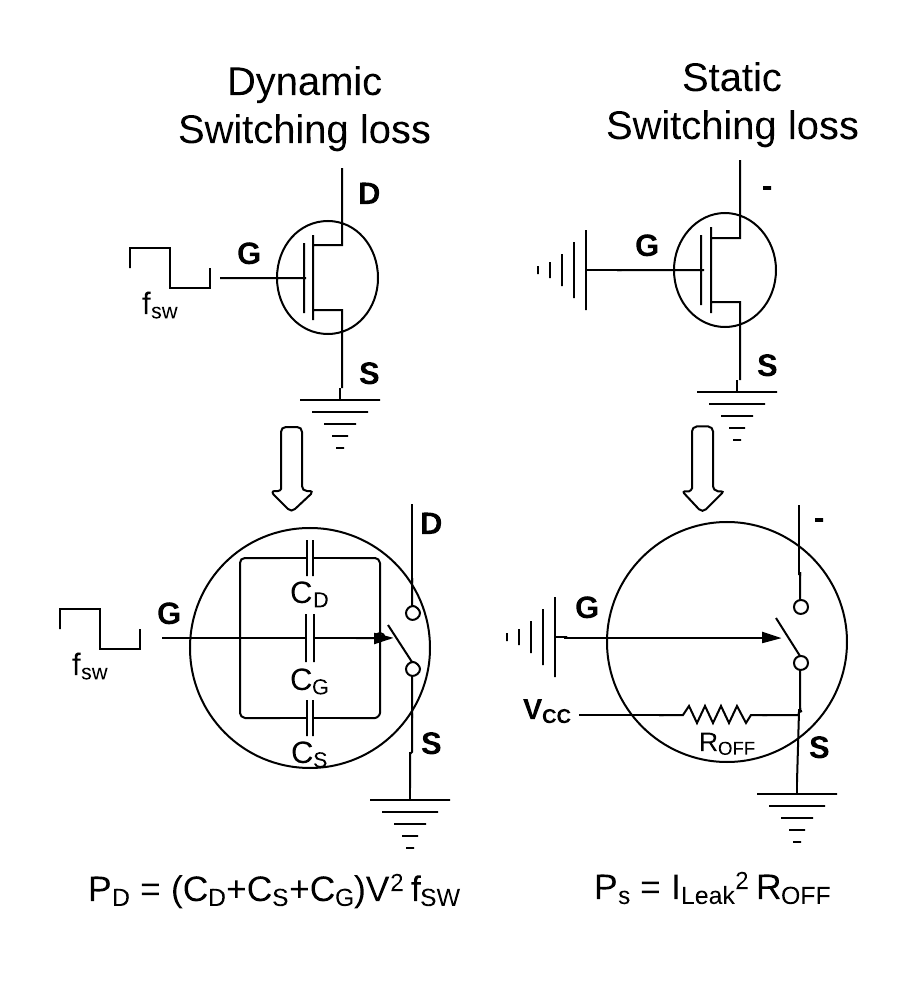
\includegraphics[width=0.4\textwidth]{SwitchLosses}
\caption{Diagram of major MOSFET switch losses}
\label{SWLosses}
\end{figure}

Static losses are constant no matter if the MOSFET switch is on or off. They occur because the MOSFET does not have an infinite open circuit resistance. Static loss is therefore technology node dependent and impossible to remove completely. Static losses are contributed to by components from sub-threshold leakage and gate oxide leakage currents.\\
These losses are intrinsic to all transistor based switches, however trade-offs possible in modern technology nodes for full integration are less optimal than older technologies. Aggressive technology scaling continuously increases transistor leakage\cite{Iwai2009}, so that realising the highest compute performance results in switches with the lowering efficiency in fully integrated designs.\\
Dynamic losses occur due to toggling the MOSFET switches. Power is consumed by changing the switch condition. As such, losses can be reduced by controlling switch toggling frequency, since for a given technology loss of the power switches and drivers increases by approximately $\sqrt{F_s}$\cite{Andreou1999}. However given fixed size energy transfer components, reducing $F_s$ reduces the converters power rating since $P = F_s \times E$.\\
Conduction loss occurs because the MOSFET switch does not have a zero on resistance. At a DC operating point, the conduction loss is simply the resistance of the MOSFET. Resistance of a MOSFET may be reduced by decreasing its channel length, $L_{ch}$ or increasing its channel width, $W_{ch}$. The minimum channel length is determined by process node e.g. $22_{nm}$ long in a $22_{nm}$ process, but channel width can be extended arbitrarily. However gate capacitance, $G_c \propto W_{ch} \times L_{ch}$. Reducing conduction loss therefore increases dynamic loss by increasing the power needed to charge $G_c$ and toggle the switch.\\  
\indent As a final note, CMOS switches cannot usually operate reliably beyond the technology node voltage. This imposes limitations on the step-down voltage ratio that can be achieved if a switch is connected between power rails. %This does not impact loss but it does mean that the power a converter can supply is maximum when the step-down ratio is $1:1$ \textbf{TRUE KINDA BUT JUSTIfy WITH EQN}\\
\indent By considering a fully optimised switch, we see the pressing research problems are reversing the leakage trend\cite{Iwai2009} and operating with rail voltages above the target technology rating.\\ 
\textbf{Capacitors: }
As previously noted, on-chip capacitors suffer particularly from bottom plate capacitance as shown in Figure \ref{BottomPlatePar}.\\
The loss problem is complicated by the frequency dependence of capacitor impedance/reactance. This is encapsulated with the capacitors "Q" quality factor. $Q_c=\frac{1}{\omega CR_c}$. If $Q_c$ = 1, the capacitor is ideal and does not impede a voltage signal. The "Q" factor has a different level of criticality in SC and buck designs. buck designs can offset a low capacitor "$Q_c$" value with their inductor if properly designed.\\
Because converters normally operate at a high frequency, Loss in the capacitor is typically due to its equivalent series resistance, $R_c$ and its parasitic capacitance $C_p$. The major parasitic capacitance component is formed between the ground node and bottom plate of the capacitor\cite{Damak2013}. This is more critical for integrated SC designs since they must transfer all of their energy via capacitors with a large area in close proximity to the ground network. As was seen in the baseline SC, failure to model losses during design can greatly impact efficiency ~\cite{Viraj2007}.\\
\indent Considering the loss mechanisms in a capacitor, improvements to integrated converters are not easily made at the architectural or circuit level if the load is heavy. Important research questions involve critical technology parameters. We also observe buck converters are less sensitive to low quality capacitors.\\
\textbf{Inductors: }Inductors, similar to capacitors suffer from frequency related non-idealist as well as static DC loss. As such, they have a quality factor, $Q_l = \frac{\omega L}{R_l}$. As in the case of the capacitor, $Q_l$ = 1 represents a perfect inductor. In a standard CMOS process, $R_l \gg R_c$. This is because $L \propto \phi_{ind}$ where $\phi_{ind}$ is magnetic flux. In standard CMOS, $\phi_{ind}$ is increased by increasing the inductor length and hence increasing $R_l$. Contemporary CMOS has metal layers optimised for digital circuits, so design rule track spacing is likely sub optimal from a flux linkage perspective. Area is inefficiently used and $R_l$ is high. Conversely for a capacitor, increasing $C$ requires increasing plate area and hence reducing $R_c$. For this reason SC designs often cite low $Q_l$ as their research motivation (~\cite{Pique2012}, ~\cite{Yogesh2010}, ~\cite{PhuckLe2011} etc.).\\
\indent Because the impedance of inductors is phase shifted from capacitors, buck converters can be optimized at the circuit level through component sizes. However, given their low $Q_l$ due to high resistive loss, important research questions concern technology parameters critical to improving $\phi_l$ and reducing $R_l$.\\    
%TODAY CONVERTERS ARE SUFFERING 65 % OF THEIR ENERGY LOSS THROUGH INDUCTORS "High-Efficiency Silicon-Embedded Coreless..."


%what is wrong with the control? \\
%What is wrong with the capacitors?\\
%.~\cite{Pique2012} evaluate the state of the art and plot an frontier of capacitor area to converter efficiency for Integrated converters. In general they find as capacitor area exponentially increases power density follows with only a linear cost in peak efficiency. However, efficiency exponentially decreases with power density in the non-ideal case. \\
%What is wrong with the inductors?\\

\section{Summary of recent literature} \label{litReview}
An evaluation of recent literature finds a volume of work addressing the previously outlined issues of baseline CMOS integrated converters.\\
We review the literature beginning with work on the common building blocks of passive components and power transistors, then move on to review system level advances.\\ 
\subsection{CMOS Switches: }Alimadadi et al.\cite{Alimadadi2008} propose an energy recycling mechanism to use the charge at the power switch gates as useful energy by pumping it to the load. The power PMOS and power NMOS gates are driven by stacked supply buffers to toggle the power switches. vss of the power PMOS gate buffer is vdd of the power NMOS gate buffer via an electrical connection at a node, $x$. by connecting node $x$ to the load via a forward-biased diode, energy used to charge power MOS gate capacitance can also charge the load node, rather than sink to ground. The drawback of this technique is that the $\frac{1}{2}$ VSS swing of the power MOS gate nodes limits the amount of step-down possible. It would therefore not translate to a high voltage step-down\\
\indent Bathily et al.\cite{Bathily2012} also focus on energy loss in switch toggling. They propose an LC tank that resonates at $F_s$ such that the power MOSFET switch gate voltages oscillate at this resonant frequency. If the power switch gate voltage is low the switching energy is stored in the tank inductor. If the power switch gate voltage is high, switching energy is stored at the switch nodes. The authors find improvements in switch efficiency ranging from around $12 - 25\%$ across the complete operating range. However the requirement is 16nH of inductance occupying 40\% extra silicon area in a standard CMOS process. The technique is applicable in high voltage converters, but the $\approx$30\% reduction of energy density makes it unattractive in medium to high power applications.\\
\indent Hyunseok et all.\cite{Hyunseok2012} address the higher than operating voltage step-down issue with circuit design and CMOS layout techniques. The circuit design handles higher than operating voltage by stacking power MOSFET devices in series such that each device does not drop more than the CMOS operating voltage. The sum of series voltage exceeds the operating voltage however. This technique is made novel with the circuit design of the power MOSFET switching inputs, which are toggled by operating voltage, despite the switch stacking. Although an arbitrary voltage step-down could be achieved with power MOSFET stacking, this technique has diminishing efficiency for two reasons. Firstly, the conduction loss of the stacked power switches is summed, reducing efficiency. Secondly the switch toggling energy of the stacked power switches is summed since it is capacitive. This reduces the maximum $F_s$ and therefore increases the required $C$ or $L$ for a fixed power envelope. As such this technique is less attractive as input voltage increases.\\
\indent In the same increased $V_{In}$ vein, Bandyopadhyay et al\cite{Bandyopadhyay2011} propose a buck converter with stacked power MOSFET switches. However, they use a single drain extended NMOS (DEnMOS) for high voltage and stacked PMOS devices. DEnMOS increases the reverse breakdown voltage of a MOSFET so that it will not short circuit at voltage above the technology operating vdd. An advantage of DEMOS is that no special process steps are needed. The main disadvantage of DEMOS in high voltage converters is high on-resistance and sensitivity to process variation. The limit of voltage step-down and current flow is around 30V at 2A \cite{Hower2005} at which point non-standard CMOS process is required for reliable operation.\\
\indent With the limit of DEMOS understood we consider the literature regarding switches suitable for high voltage and or high current.\\
For voltages above 20V at current above 1A, LDMOS switches outperform DEMOS. Hower et al\cite{Hower2005} are paraphrased as follows: \textit{LDMOS devices have lower on-resistance than DEMOS but have a fixed device length, so transistors cannot be folded geometrically}. LDMOS can be integrated into a low voltage technology node monolithically because they are compatible with bulk CMOS. The cost is an additional mask layer and therefore a non-standard process. A final drawback is LDMOS has a higher $V_t$, so they require more switching energy.\\
\indent Finally in the high $F_s$, high power design corner we consider AlGaN/GaN switches. Although much research effort has been made to improve power density and breakdown voltage, AlGaN/GaN switches outperform LDMOS in high-power high frequency switching applications \cite{Goyal2013}. This is because these switches have unique semiconductor properties beneficial to high voltage power conversion, such as; high operating frequency, high current density and high breakdown voltage\cite{Alamo2009},\cite{Mustapha2008}. Krausse's\cite{Krausse2013} summary of recent literature on power transistors is reproduced in Figure \ref{GaNCharacter}. This graph demonstrates the advantages of AlGaN/GaN devices over LDMOS in the high power domain.\\ %The Goyal2013 says that AlGaN dominate LDMOS in high bandwidth high power applications such as optics and in base stations It is also later than this: http://www.microwaves101.com/encyclopedia/ldmos.cfm which questions AlGaN/GaN
\begin{figure}[here]
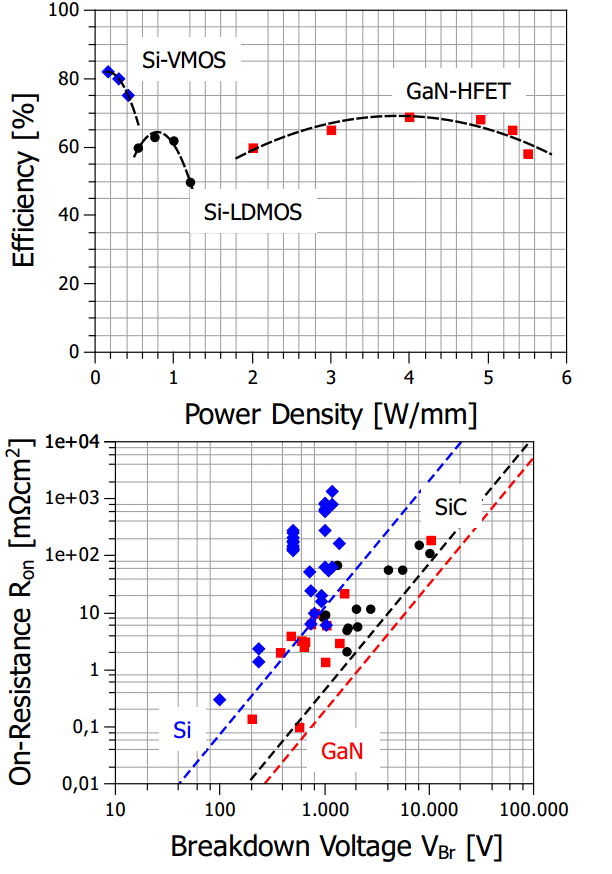
\includegraphics[width=0.4\textwidth]{TransistorPerf}
\caption{Comparative performance of power switch types, Reproduced from\cite{Krausse2013}}
\label{GaNCharacter}
\end{figure}


\indent To conclude discussion on power switches, the literature proposed novel circuit designs to improve switching efficiency. The limitations of these designs focus attention on the switch devices. The literature indicates as voltage and power density demands of a design increase, non-standard CMOS process and CMOS alternatives become increasingly attractive.\\
\subsection{Capacitors: }After Viraj et al.\cite{Viraj2007}, much research effort was expended regarding converter capacitor energy density and impedance modulation. Kwong et al.\cite{Kwong2009} address both issues uniquely. The load is a sub-threshold processor, which allows low-energy density capacitors to provide adequate drive. Converter impedance is reduced with technology options and circuit topology. Metal insulator metal (MIM) capacitors are used as power passives. MIM capacitors have the desirable qualities of being compatible with bulk CMOS and having a high $Q_c$. Their disadvantage is low energy density.\\
With low energy density, impedance matching becomes increasingly important for a converter to have compelling performance. Viraj et al.\cite{Viraj2007} observed an exponential deterioration of efficiency with mismatched load impedance. % This work implements a re-configurable step-down voltage circuit, where output capacitors can be stacked for 4 step-down voltages or 4 converter impedances.\\
%Kwong et al. stands alone in the literature because it uses a sub-vt processor load to mitigate low energy density where most literature attempts to improve it.\\
\indent To revisit energy density, non-standard CMOS capacitors dominate contemporary integrated converter literature. Since energy density is improved by reducing loss, early work explored the limit of CMOS with circuit techniques. Besides their other innovations, Kwong et al.\cite{Kwong2009} feature a charge recycling circuit. The operating principle is similar to Alimadadi's work\cite{Alimadadi2008}, but the energy source is parasitic capacitance and bond wire inductance. The technique was not implemented in later designs by the authors or others, so it is assumed to be a dead end.\\
\indent Later work focuses on technology options for improving energy density. In CMOS compatible technologies, MIM~\cite{Kwong2009} and Thin-gateMOS/fringe metal~\cite{Pique2012} capacitors are succeed by the exotic Deep trench~\cite{Pique} and Ferroelectric~\cite{Damak2013} capacitors as seen in Table\ref{PermittivityTable}.\\
Exotic capacitor types typically greatly increase $C$ per unit area because they realise an extremely high permittivity ($\epsilon_r$). Capacitance may be calculated $C = \epsilon_r \times \frac{A_p}{l_p}$ where $A_p$ is the area of capacitive plates and $l_p$ is the separation distance. 
\begin{table}
    \begin{tabular}{|l|l|l|}
    \hline
    Capacitor               & Material & Permittivity ($\epsilon_r$) \\ \hline
    Bulk CMOS~\cite{Robertson2004}               & SiO2     & 3.9          \\ \hline
    High K CMOS~\cite{Robertson2004}             & HfSiO4   & 11           \\ \hline
    *Deep trench (structure)~\cite{Johari2009} & PZT      & 1000         \\ \hline
    *Ferroelectric~\cite{Lee2004}			& BaTiO3      & $\approx$4600         \\ \hline    
    \end{tabular}
    \caption{Table of capacitor permittivity where: \textit{* example technologies, not used in reviewed designs}}
    \label{PermittivityTable}
\end{table}
%\textit{* example technologies, not used in reviewed designs}
High $\epsilon_r$ can effectively negate bottom and top plate parasitic capacitance, since these parasitic capacitors could have an $\epsilon_r$ several orders of magnitude lower than the power capacitors.\\ 
To close on the topic of high $\epsilon_r$, Deep trench and Ferroelectric capacitors designs do not exhibit multiple order of magnitude power density improvements over others. In these technologies, $\epsilon_r$ varies with greatly with temperature ~\cite{Lee2004} and frequency ~\cite{Callister2012}. %http://www.mrl.ucsb.edu/~seshadri/old/MATRL100A/class13.pdf
Further research is needed to understand their limits in power converters.\\
Another class of converters has gained prominence due to the difficulties of energy density in capacitors. Semi-integrated converters (~\cite{Pilawa2012}, ~\cite{Bathily2012}, ~\cite{Ng2012} etc.) use off-die capacitors as a charge source. Provided such capacitors can be connected to the rest of a converter with a very low inductive path, these designs offer higher drive capability at the cost of an extra component.\\
\indent In summary of capacitors, early CMOS circuit level approaches to energy density have been superseded by non-standard CMOS. %Architectural level approaches in SC designs have been successful in improving impedance modulation.\\
\subsection{Inductors: }Since total inductance is improved by increasing mutual inductance within a conductor structure, researchers have made several attempts to improve $Q_l$ with custom inductor layout. Angular spiral inductors were shown to have inadequate $Q_l$ for efficient fully integrated power converters\cite{Alimadadi2008},\cite{Artillan2011}, motivating exploration of alternate structures and materials. Meere et al. \cite{Meere2009} characterized fully integrated racetrack style inductors for buck power converters. They find the $Cu$ resistivity to dominate loss and to increase exponentially with $F_s$. They conclude 7mA as the supply limit of a converter with such inductors.\\
As with capacitors, the $Q_l$ problem was also explored using semi-integrated converters. Researchers realised the parasitic inductance of bond wires could be re-purposed to become active power delivering inductance~\cite{Wens2007},~\cite{Ahn2012}. This work received much attention owing to the high $L$ of bond wire relative to integrated $Cu$ spiral and racetrack inductors. In addition, since package inductance is a large contribute to power loss, end to end efficiencies have been realised up to 84.7\%~\cite{Cheng2013}. Owing to the relatively low resistivity of bond wire, energy density is also greatly improved with an $I_{Out}$ of 1.2A reported~\cite{Cheng2013}.\\
\indent Researchers have also combined innovations. $L$ is enhanced when the core of an inductor is a high permeability material. $L \approx \frac{N^2\mu A_L}{l_L}$ where $\mu$ is the permeability of the core. To this end Hongwei et al.~\cite{Hongwei2011} propose applying a ferrite epoxy to bond wire inductors, with Wang et all. proposing ceramic tape for 2.5D semi-integrated passives. Although neither author was able to match the energy density of Chengs work, a more fundamental issue omits bond wire inductor converters as a candidate technology for pin optimisation. Consider the example pin configurations in Figure\ref{BondWireLim}.
    
\begin{figure}[here]
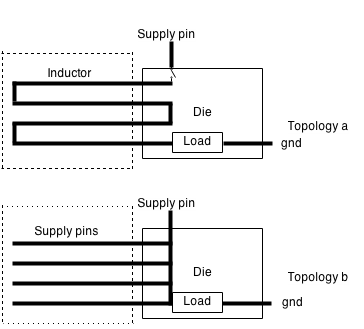
\includegraphics[width=0.4\textwidth]{CostvsGainofBondWireInductor}
\caption{The power limitation of bond wire inductors}
\label{BondWireLim}
\end{figure}

Operating at the current failure limit and given that $\eta < 100 \%$, Topology b, with no switching converter in Figure \ref{BondWireLim} is able to deliver more power per pin than topology a, which features bond wire inductors.\\
\indent With the above mentioned limitations, research integrating high permeability materials into custom layout inductors is considered. Recent advances in device physics have yielded thin film inductors ~\cite{OSulivan2013} with orders of magnitude energy density improvement over those in prior art~\cite{Meere2009}. Sturcken et al.~\cite{Sturcken2013} propose a converter with such devices able to drive 6.3A and Intel report 400A~\cite{Intel2010} using the same inductor technology. This is the highest reported drive of all integrated converters to the authors knowledge. Thin film inductors are presently subject to a caveat. Due to their geometric structure and unique ferroelectric core they are not integrated into bulk CMOS in the literature, instead being built on a separate interposer.\\
\indent Inductor research is summarised as being a focussed effort to improve $Q_l$. The state of the art is represented by thin film inductors, which enable much higher energy density converters than capacitors alone.\\


\indent Component literature as a whole is distilled as follows; power switches offer many options for design trade-off, depending on the operating requirements of a digital circuit. The upper limits of voltage and energy density are reached with CMOS alternative transistors. Passive components were limited in energy density with standard CMOS. Recent advances in device physics have succeeded in miniaturising energy dense inductors and capacitors, but these require additional doping material and process steps to create on bulk Si. As with power switches, the upper limit of energy density is not demonstrated in bulk CMOS\\
%DONT SKIP CONTROL PAPERS, NEED TO TALK ABOUT DCM MODE FOR LIGHT LOAD (NOT DEFINED EARILER) THEY DONT REALLY ADD MUCH 

\subsection{SC Architecture}
Integrated SC architecture research focusses on addressing the poor load regulation and line noise of the basic circuit topology described earlier.\\
\textbf{Improving load regulation: }Basic SC converters have no load regulation. Load regulation is desirable as it improves the exponential decay in efficiency outside of the basic topology operating point(s). This is because increasing $Z_O$ for light loads means less power is burned in the converter, since for a fixed operating voltage, the end to end DC impedance is higher and therefore end to end DC current is lower.\\
\indent As seen in  Viraj et al.~\cite{Viraj2007} Integrating SC converters to digital processor dies allows for complex capacitor and switch topologies, since bulk capacitance can be sub-divided.\\
Le et al. \cite{Phuck2010} propose a novel converter circuit topology with more granular impedance modulation control than that of Viraj. By splitting $C$ into 4 parallel SC converter modules, $Z_O$ is adjusted by modulating the phase difference between the $F_s$ of these modules. The converter also features the re-configurable step-down voltage circuit for coarse grain voltage control reported in Kwong's work ~\cite{Kwong2009}. Peak efficiency is far higher than Viraj's work\cite{Viraj2007} at 82\%, and the efficiency curve has linear regions as opposed to the purely exponential worsening of Viraj.\\
Although other work (~\cite{Ramadass2010} etc.) implements capacitance modulation, Le et al. is notable for additionally implementing switch conductance modulation.\\
Conductance modulation of the power switches allows finer control of converter impedance, since the MOSFETs are analogue devices. However since the operating principle is equivalent to an LDO, it is unattractive in terms of efficiency.\\ 
\textbf{Improving line noise: }Basic SC converters have high voltage ripple because of exponential discharge of the power capacitors to the load. Improving the voltage line stability is important as digital circuits have low line noise tolerances.\\ 
Line noise is addressed in the literature by sub-dividing the load driving capacitance as was seen in load regulation improvement techniques. However the capacitance visible at the load is not modulated. Instead, the converter modules operate out of phase, superposing their exponential voltage discharges on the power bus to smooth $V_{Out}$. Success of this technique motivated aggressive exploration of capacitance module phase slicing in the literature. Pique~\cite{Pique2012} reports a load driving capacitance sliced into 41 phase shifted parallel converters and find line noise to improve around 16$\times$ compared with 10 phase prior art.\\ 


\subsection{Inductor buck architecture}
The basic buck topology offers superior impedance modulation relative to SC designs by employing pulse width modulation (PWM) of $V_{In}$. Earlier discussion focussed on Continuous current mode (CCM), where conductance is varied by altering the duty cycle $D$ of the switch at $V_{In}$ in Figure \ref{BKTopology}. Increased conductance improves buck voltage droop for heavy loads since the converters impedance can be reduced for power transfer at a maintained operating voltage as the load increases.\\
For light loads, efficiency is improved with increased Impedance. Impedance is increased by shortening the inductor charge pulse. In DCM, inductor current is "discontinuous" because the charge pulse in the PWM is so short the inductor fully discharges into the filter capacitor $F_c$ and load. In DCM mode, DC $V_{Out}$ is no longer simplified to $D \times V_{in}$ because $C$ supplies both current and voltage after the inductor is discharged. Resolving $V_{Out}$ is therefore non trivial for buck control circuitry.\\
\indent Integrated buck converters can feature complex digital control loops and the literature explores this space. The two challenges are precisely controlling the operating point in DCM and switching between DCM and CCM at optimum intervals for a load in flux.\\
Wens et al. ~\cite{Wens2011} report a novel SCOOT control system for alternating between CCM and DCM. SCOOT differs from the bulk of literature on this topic by splitting the passive components into a grid of sub modules, a technique applied in integrated SC architectures. However unlike capacitance, inductance reduces for electrically parallel modules, such that the 4 constituent converters quiesce in DCM mode. The superposition principle allows Wens to simulate CCM in this quiescent mode by adding a phase shift of $\frac{\pi}{2}$ for each module relative to its two adjacent neighbours. DCM can be forced by reducing the duty cycle $D$. The benefit of this approach is reduced ripple voltage at $V_{Out}$ compared with monolithic passives. SCOOT varies module phase along with $D$ in attempts to optimize the operating point to load, however the latency of the passives and control circuitry appears to oscillate efficiency around the load operating point in an undesirable way.\\
\indent The imprecise operating point of DCM is addressed with control techniques on monolithic passive designs.\\
DCM control operates on a hysteresis principle since $D$ does not govern $V_{Out}$ in DCM mode. Non-integrated buck converters can adjust $T_{On}$ of the power train switch(es) after sensing $V_{Out}$ in a timely fashion since these converters feature large passive devices. Switching speeds typically occur in the KHz regimen. The small passive size of integrated converters requires switching speeds of hundreds of MHz (~\cite{Alimadadi2008}, ~\cite{Bathily2012}, ~\cite{Sturcken2013} etc.). With control circuit blocks operating in the nS range, simple hysteresis control of integrated bucks has received attention in the literature.\\
Feng et al.~\cite{Feng2008} propose a delay compensation hysteresis controller for integrated DC DC converters, however their approach requires overcharging the load for faster operation of the control comparator circuitry. This is unattractive from an efficiency perspective, since the goal is to increase converter impedance in DCM. Cheng et al. ~\cite{Cheng2013} address this by using a short discharge pulse of the load. They calibrate the control loop timing for different light load conditions using difference in the sensed $V_{Out}$ before and after discharge to determine an optimum $T_{On}$ to restore $V_{Out}$. As Cheng's method increases output impedance, it is more attractive in DCM mode than Feng's. The 84.7\% efficiency is the highest reported for a chip integrated buck converter, however the architecture cannot be applied to moderate and heavy loading conditions.\\  
\indent Researchers have applied circuit design to improving performance characteristics besides efficiencies. An additional flying capacitor added to the basic circuit can reduce the total capacitance by 50\% according to Cheng~\cite{ChengII2013}. Flying capacitor buck converters vary in topology depending if the target passive for reduction is capacitive ~\cite{ChengII2013} or inductive ~\cite{Kim2011}, but all create a more complex filter and energy storage network. The Additional components allow greater freedom in creating the circuit transfer function enable researchers to operate at a target load range with smaller passives, by focussing filter attenuation to the switching frequency more precisely.\\

To summarize converter architecture research, integrated buck and SC topologies improve performance with common techniques such as passive slicing and control phase shift techniques applied to modular converter designs. Both types of converter are able to improve control of impedance, $Z_O$ however the SC design is still fundamentally limited to higher impedance than the buck.\\
In addition, circuit techniques in the literature are shown to reduce the passive sizes beyond those required for a basic topology.\\  
 
%\textbf{System: well defined, class of problems: well defined, now we will see "fixed" systems}\\
%\begin{itemize}
%\item{Switches fixes paper list and description DONT USE EXOTIC TECH! THESE WERE NEVER USED ON INTEGRATED DESIGNS!!!}
%\item{Control fixes paper list and description NOTE THAT THIS PROBLEM IS WELL UNDER CONTROL, CONCLUDE FROM THIS SECTION} Le note that splitting $C$ into parallel converter modules improves the terrible ripple of SC converters, 41phase of Pique takes this to the next level. all those phases greatly smooth ripple but this is an architecture/control technique
%\item{Capacitor fixes paper list and description NOTE THAT THIS PROBLEM CANNOT BE "SOLVED" FROM A SC TOPOLOGY POINT OF VIEW AND INDUCTORS ARE "BETTER" IN TERMS OF ENERGY DENSITY AND LINE REGULATION. Note faliures: MIT charge recycling work did not work!. Figured out loss conditions capacitors here: A 32nm Fully Integrated Reconfigurable Switched-Capacitor DC-DC Converter Tried to mitigate bottom plate parasitics with fractal caps.defined here:\cite{Samavati2008} but not the paper }
%\item{Inductor fixes paper list and description. NOTE THAT THIS IS "SOLVED" BUT FOR SEMI-INTEGRATED OR WHATEVER note topology fixes, flying capacitor is used}
%We note that the approach is not necessarily to increase the size of inductance, but the quality factor. the baseline CMOS \cite{Alimadadi2008} realized 4.38nH inductors which is comparable with \textbf{Guys} at \textbf{5.NHS}, but the later work is able to realize a far greater energy density due to the novel technique of using bond wire as inductors.
%\item{SC Ripple Fixes} % Fully Integrated Capacitive DC-DC Converter wit all digital Ripple Mitigation technique
%\end{itemize}

\section{The IO limit with integrated DC DC converters}

High performance IO pins in digital circuits have a bandwidth constrained by both the electrical performance of the transmission line and IO buffers. Given the previously reviewed literature on the state-of-the-art of integrated DC DC converters, this section considers the possibilities of mitigating IO bandwidth limiting factors using integrated DC DC converters.

\subsection{DC DC converters and IO pin performance}

For a given SOC design if power were supplied independently from the die substrate, the IO bandwidth limit of the pins on a chip package is defined by signal integrity limits. The theoretical limit proposed by Shannon~\cite{Shannon1948} defines an SNR that must be met for information transfer. For some given noise, chips toggle their pins with an SNR headroom beyond Shannon's limit for practical IO circuits. As frequencies increase it becomes more difficult to maintain this headroom. The reason is characterised by 
\begin{itemize}
\item Reducing signal drive relative to noise
\item Increasing signal attenuation relative to noise
%\item Signal noise
\end{itemize}


For signal attenuation consider the transmission line diagram, Figure\ref{TXLine}\\
\begin{figure}[here]
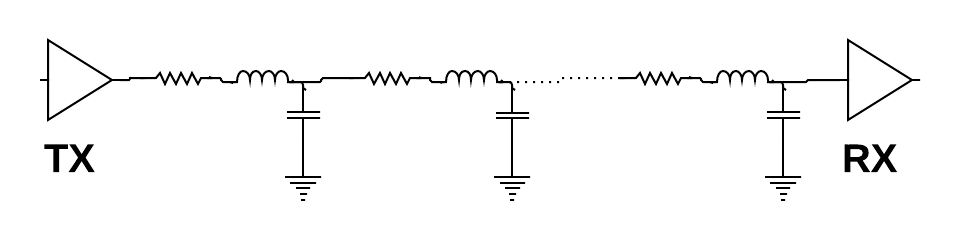
\includegraphics[width=0.4\textwidth]{TransmissionLine}
\caption{Transmission line model with parasitic $Z$}
\label{TXLine}
\end{figure}
We see that the parasitics create a low pass filter on the transmission line. A high IO transmission frequency offers high bandwidth but also suffers higher attenuation along the line. Because noise has constant power for all frequencies, the result is lower SNR after the noise superposes with the IO signal at the IO receiver terminal. Since the parasitics increase in value with line length, transmission lines may be shortened to reduce filtering and improve SNR. The parasitics are also affected by transmission line electrical quality so filtering is also reduced with routing techniques for common mode noise rejection and improved materials with lower capacitance and inductance per unit volume.

For reducing signal drive consider the IO buffer diagrams, Figure\ref{IOBuf}\\ %http://www.ti.com/lit/ds/slls003e/slls003e.pdf
%Pre-charge http://www.eecs.berkeley.edu/~yidaduan/EE241_report.pdf
\begin{figure}[here]
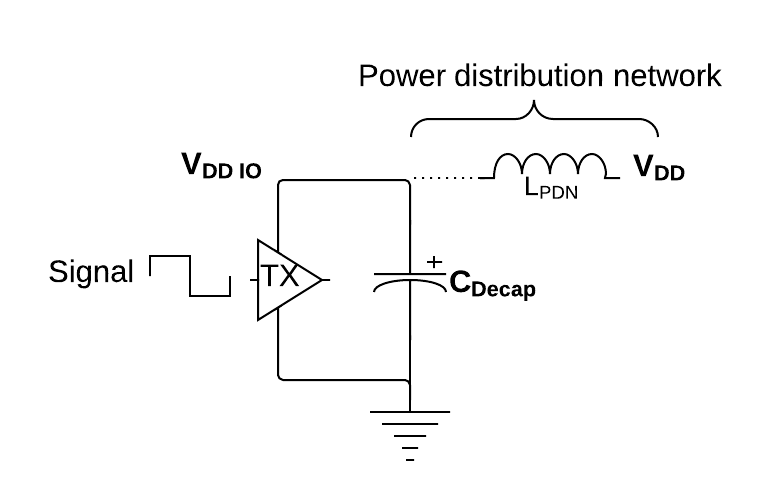
\includegraphics[width=0.4\textwidth]{IOBufferDroop}
\caption{Power route of an IO buffer}
\label{IOBuf}
\end{figure}
A high IO switch frequency will deplete the local charge well and reduce the IO buffer supply voltage. 
The supply voltage of buffers must be maintained for the maximum buffer output swing and hence maximum SNR of IO. Consider the difference in system topology for integrated and external DC DC Converters in Figure \ref{DroopTop}\\
\begin{figure}[here]
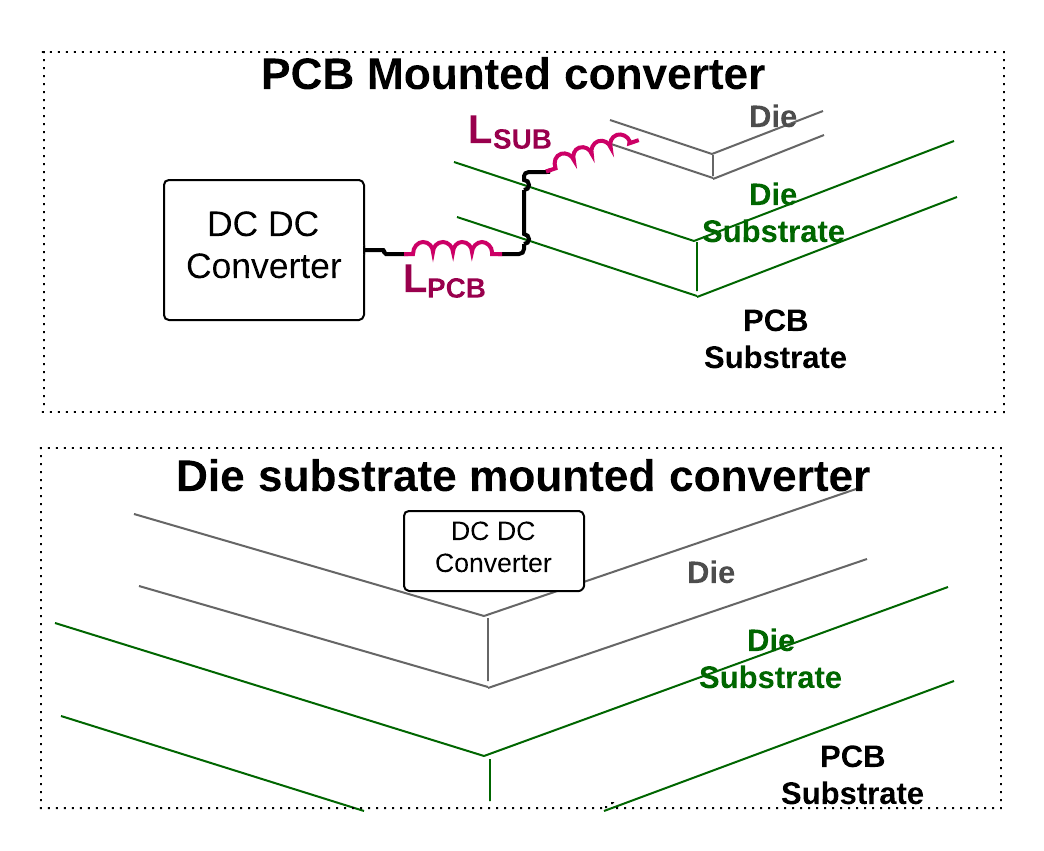
\includegraphics[width=0.4\textwidth]{DroopResponseLatency}
\caption{Inductive path between converter and load}
\label{DroopTop}
\end{figure}
The high switching speed and bursty nature of high speed IO, such as processor to processor interfaces creates a performance corner requirement for DC DC converters. For reliable chip operation, the converter must be able to respond to transient I$\times$R drop at the IO buffers $V_{CC}$. Because of the long control sense and signal path between an off chip converter and IO buffer, large parasitic inductance along this connection increases delay in this power converters response time to transient I$\times$R drop. This delay attenuates IO signals by reducing the drive strength of IO transmission buffers and reduces SNR.\\

A review of Intel processors from the past three decades evidences aforementioned SNR challenges in high speed IO.
Processor IO bus width and frequency increased significantly from the Intel 4004 to pentium chip. Subsequently bus frequencies increased steadily but bus width did not significantly increase until the 2nd Generation Core processor, when the parallel FSB was replaced by the narrower differential QPI bus. Beside pin counts and toggle speeds, the consistent shrinking of FSB routing lengths, increasingly stringent demands on PCB materials and the eventual full switch to differential high speed IO evidence increasing difficulty over the years to maintain SNR at IO receivers in advanced digital circuits.\\ %\textbf{NEED TO MASSAGE THESE NUMBERS!} 
\textbf{Addressing SNR: }
Signal attenuation relative to noise is beyond the scope of DC DC converters as it depends on PCB routing, however converters can improve SNR from the perspective of drive strength and potentially push the IO limit of a digital chip.
%Integrated DC DC converter can improve SNR to and the IO limit\\
\indent As mentioned, IO drive strength is compromised because of localized transient voltage droops at IO driver transistor supply terminals. %This reduces the SNR since the IO buffers have a weaker drive capability. 
Not only can integrated converters respond faster to voltage droop than external converters, they may do so on localised regions of a power grid. Designs such as the previously noted Wens buck~\cite{Wens2011} split the power components into modules distributed geographically in a chip. Similarly distributed $V_{Out}$ terminals and localized control loops could actively address regions of transient $I \times R$ droop.\\ 
%\indent \textbf{Signal attenuation: }
%An integrated DC DC converter addresses the problem of transient IO loading. The inductance path from power supply to IO buffer $V_{CC}$ is reduced. This makes reliable chip operation easier to achieve, since the on chip converter can respond to transient I$\times$R drop faster. The granularity of transient I$\times$R drop is also improved since the on chip converter can be split into multiple power supply modules driving regions of the power distribution network. The literature exemplifies several such topologies \textbf{CITE}. 


 
  
%\textbf{Defines stakeholder specific problem}\\
%Think about this, it has to be differentiated from the section above

\subsection{Saving pins with DC DC converters}

The literature demonstrates integrated power converters capable of replacing external VRMs. A small subset of this literature considers input voltage above those common to Li-Ion batteries. 
\indent Although the component literature and select converter architectures identified in section \ref{litReview} show promise for application to this problem, many combinations from this collection of parts have not been explored. Therefore the performance of integrated converters in high voltage is an open research question

Practical high power, high voltage integrated converters are the enabler for pin count optimisation as they define the lower bound of pins required for a given power envelope.\\
Previously reviewed literature finds active and passive components capable of driving a spectrum of processor power loads. reviewed literature has also reported integrated converters capable replacing external VRMs. However up to this point the report has focussed on systems operating at input voltages of $4.5V$ and lower. With high voltage switches reviewed, state of the art in high voltage integrated converters are reviewed in this section.\\

\indent As high power density passives are nascent, there is a dearth of literature on high voltage integrated converters owing to their impracticality as LDO replacements. Two representative designs are reviewed below that attempt to circumvent the limitations of commonly available low power integrated passives.\\
\textbf{High voltage SC-buck: }Pilawa et al.~\cite{Pilawa2012} Implement a twin stage step-down converter that is a hybrid SC and buck design. high voltage input is stepped down by an SC phase as pre-regulation. The output of the pre-regulator is input to a secondary buck phase, which cleans the noisy SC voltage with its filter and provides an analogue range of low voltages.\\
Pilawa et al. ~\cite{Pilawa2012} implement a semi-integrated design. They achieve relatively high power density of 0.8W with off die passive components. High input voltage is handled with LDMOS (triple well) switches, which increases the operating voltage at the cost of switching speed. Since the buck stage operates within nominal bulk supply voltage, its power switches operate much faster. This improves the realisable $Z_O$ regulation speed.\\
The LDMOS switches are a technology option of the CMOS process chosen in the work. They limit the design input voltage to 5V and are a significant source of loss.\\
With more closely integrated passives and improved switches, the ideas of this work could mature into a practical candidate for high voltage integrated power converters.\\
\textbf{High voltage substrate transformer-buck: }High voltage DC DC converters (5v+) miniature power converters exist as PCB substrate integrated devices. With semi-integrated converters emerging as viable replacements for off chip VRM's, we consider the limit of semi-integration. Much of the reviewed literature integrates passive components on to die substrate (~\cite{Pilawa2012}, ~\cite{Bathily2012}, ~\cite{Ng2012} etc.). Gong et al.~\cite{Gong2008} is an example of substrate integration for high voltage, high energy density power converters. The design embeds a miniature transformer coil and inductor coil in a 6 layer PCB substrate. The control IC, power switches and capacitor are mounted on this substrate. This design operates in the high voltage high power, high efficiency corner. Metrics are respectively 48V, 300W and 96\% peak.\\
This level of substrate integration and power output has several drawbacks. The primary issue for pin count optimisation is substrate area consumed by planar power components blocks vias and constrains pin routing.\\
Designs such as that of Gong offer a potential means for high voltage efficient converters but have a high component cost and area penalty in the substrate. This limits their appeal for increasing pin count, despite their demonstrated utility in supplying power.\\       
\indent To conclude on the state of the art, a lack of exploration in high voltage integrated converters was identified. Practical semi-integrated approaches were found but have limited power capabilities or limited appeal for pin optimisation. 
%\textbf{Solutions \& Stakeholders, why is there still work to be done?}\\
%Need to define the problem of Signal to power pin ratio. We cannot optimize this today with DC DC converters, because the \@ CMOS voltage step down means we need to have a lot of CORE power pins.\\
%Our stakeholder" is high voltage step down If we do it we could reduce \textbf{DEFINE}"CORE POWER PINS" to an amount desirable for \textbf{DEFINE} signal integrity\\
%Now we can outline the high voltage work that was summarized in the google doc I did

\subsection{Directions for future work}

An evolutionary comparison of work is presented in Table \ref{EffnEnergyDensity}.\\
%\begin{table*}[t]
%\centering
%    \begin{tabular}{|l|l|l|l|l|l|}
%    \hline
%    Design                  & Converter type           & Integration & Special tech                         & Efficiency   & Energy density \\ \hline
%    SC inductor buck~\cite{Pilawa2012}        & SC buck           & Semi        & Unknown                              & 81\% peak    & $0.08W/mm^2$    \\ \hline
 %   Substrate transformer~\cite{Gong2008}   &  transformer buck & None        & none                                 & 96\% peak    & $1.5W/mm^2$*    \\ \hline
  %  CMOS buck~\cite{Wens2011}               & buck                     & Full        & none                                 & 58\% peak    & $0.2W/mm^2$     \\ \hline
   % Bond wire buck~\cite{ChengII2013}           & buck                     & Semi        & none                                 & 82.4\% peak  & $0.86W/mm^2$    \\ \hline
    %Thin film inductor buck~\cite{Sturcken2013} & buck                     & Semi        & Interposer \& thin film inductors & 69\% nominal & $22.6W/mm^2$    \\ \hline
    %\end{tabular}
    %\caption{\textit{*reduced to two dimensions by dividing over depth of substrate}}
    %\label{EffnEnergyDensity}
%\end{table*}
\begin{table*}[t]
\centering
    \begin{tabular}{|l|l|l|l|l|l|}
    \hline
    Design                  & Converter type           & Integration & Special tech                         & Efficiency   & Energy density \\ \hline
    Substrate transformer~\cite{Gong2008}   &  transformer buck & None        & none                                 & 96\% peak    & $1.5W/mm^2$*    \\ \hline
    CMOS buck~\cite{Wens2011}               & buck                     & Full        & none                                 & 58\% peak    & $0.2W/mm^2$     \\ \hline
    Bond wire buck~\cite{ChengII2013}           & buck                     & Semi        & none                                 & 82.4\% peak  & $0.86W/mm^2$    \\ \hline
    Thin film inductor buck~\cite{Sturcken2013} & buck                     & Semi        & Interposer \& thin film inductors & 69\% nominal & $22.6W/mm^2$    \\ \hline
    SC inductor buck~\cite{Pilawa2012}        & SC buck           & Semi        & Unknown                              & 81\% peak    & $0.08W/mm^2$    \\ \hline    
    \end{tabular}
    \caption{Evolution of integrated DC DC converter circuits \textit{*reduced to two dimensions by dividing over depth of substrate}}
    \label{EffnEnergyDensity}
\end{table*}
Moving beyond these works we define a research goal of high voltage, efficient and energy dense integrated power converters for investigating the lower bound power to IO pin ratio of digital chips.\\
%Several enabling works were identified in the literature to explore this space. Therefore the goal is refined as investigating the lower bound power to IO pin ratio of realisable converters.\\
Several reviewed converter implementations can be eliminated given this goal:
\begin{itemize}
\item{\textbf{Standard CMOS SC/Buck converters: }Standard CMOS converters do not operate efficiently enough to reduce the power to IO pin ratio}
\item{\textbf{Mini-transformer: }Planar substrate transformer and inductors block both IO and power pins }
\item{\textbf{Bond wire inductors: }Consuming substrate pin pads for power inductors can never reduce the power to IO pin ratio}
\end{itemize}   
%Here we have to talk about:\\
%3 the micro transformer solution to this problem (it could be made promising) \\
Some augmentation to the reviewed literature is now postulated.\\
\subsubsection{LDMOS High voltage SC-Buck}
Pilawa's work ~\cite{Pilawa2012} Is a potential application for relatively slow switching high voltage LDMOS.\\
LDMOS transistors cannot operate fast enough to provide the tightly controlled converter required for high bandwidth IO, neither is an SC converter suited to an efficient transient load regulation. However the pre-regulated capacitors are excellent charge wells for decoupling. This allows a faster switching buck regulator to provide a clean voltage with fast transient response, since there is negligible inductance between the charge well and filter. This is the main advantage of such a design.\\
Realizing the potential benefits require several research questions be addressed.\\
\textbf{Power Density: }Pilawa's semi-integrated solution to the power density issue of integrated capacitors may be questioned and alternate avenues explored. Although power density of Pilawa's work is relatively high it is below that of Cheng ~\cite{Cheng2013}, Strucken ~\cite{Sturcken2012},~\cite{Sturcken2013} and other semi-integrated converters. As such Pilawa's power density is presently unattractive. The semi-integrated approach of passives may also be further explored as Pliawa's design mounts the power capacitors to the die substrate, introducing a far larger parasitic impedance than Sturcken and Intel's $Si$ interposer mounted inductors. The trade-off in energy density and charge cycle periods of deep trench~\cite{Pique2012} and ferroelectric capacitors~\cite{Damak2013} employed by El-Damak and others could be weighed against those of substrate and interposer mounted power capacitors.\\   
\textbf{Efficiency: }The design has a double power train and therefore double parasitic losses. The design is also complex for component value optimization since the SC and buck create a complex filter.\\  
\subsubsection{GaN Interposer buck: }Silicon interposer bucks represent the state of the art in performance ~\cite{Intel2010},~\cite{Sturcken2013}. In addition the interposer enables IO optimisation to be explored aggressively via the directions of 3D and 2.5D integration.\\
Although the $Si$ interposer design has an attractive output operating point envelope, research questions relating to its regulation capability of high voltage $V_{In}$ should be addressed.\\
\textbf{Power Density: }The question of high voltage input may be explored via the 2.5D space of the $Si$ interposer. Energy dense non standard passives and high voltage power switches reviewed in section \ref{litReview} could be used to investigate an optimum pin ratio for high $V_{In}$ whilst retaining a standard CMOS digital die. The performance of GaN switches and Ferroelectric deep-trench capacitors alongside thin film inductors is as yet unknown. All of these technologies could feature in a single integrated converter with an aggressive application of the interposer\\ 
\textbf{The limit of IO density: }A tangential exploration of processor IO density levering interposers is presented by Gokul et al. ~\cite{Gokul2011}. Interposers are used to reduce memory IO pins on the die substrate by sandwiching a Si interposer between memory and digital logic. The interposer mounted inductors used by Strucken and Intel could be integrated into such an interposer, with the buck converter used to optimise the IO and memory bandwidth to digital logic.\\
However, the weakness of the interposer buck with respect to a SC-Buck is its lack of a large local charge well, making the design rely on traditional decaps on the digital CMOS chip to mitigate transient $I \times R$ droop. A line of research inquiry may address this with the energy dense capacitors reviewed in Section \ref{litReview}.\\ 
       
%1 the disruptive technology of Si on Insulator, and how it could be paired with interposers\\
%In the mobile segment Silicon interposers can be used to solve the IO problem as seen in [Ultra-high I/O Density Glass/Silicon Interposer for high Band-witdh Smart Mobile Application].\\
%This interposer allows signal integrity to be maintained at low voltage from the interposer to memory. a High voltage from the substrate and DC DC converter integrated to the interposer allows power density to be met with fewer pins on the package. In this scenario, the package can be made smaller to allow denser integration, or the io bandwidth  can be bound to signal integrity requirements...\\

\section{Conclusions}

Integrated step-down DC DC converters show promise as a means to optimise IO pins in terms of count and performance for high performance digital CMOS chips. Integrated converters may improve power efficiency and power integrity for digital circuits and IO buffers as well as reducing the required number of core logic supply pins. The state of the art demonstrates some of this utility, but research is required to explore the full potential of integrated converters.\\  
The limits of converter circuits and their components along with related research were reviewed.\\
Novel solutions and techniques applied to these limitations show potential in addressing the efficiency and energy density issues of integrated converter circuits. However the question of optimally integrating the reviewed work for a given digital CMOS chip design remains open owing to the dearth of collaboration between specialists in each problem area.\\
\indent With a goal of IO pin optimisation, conjecture is offered on advancing knowledge in the area based on the SNR problems of high speed IO and the reviewed work. The low latency $I \times R$ droop response and high quality output regulation required may be possible by furthering the twin stage converter work of Pilawa~\cite{Pilawa2012} as this architecture features a coarse grain low latency charge well in the SC phase in support of a low drive strength high quality output line in the buck phase.\\
Alternatively, the better performing interposer buck of Sturcken ~\cite{Sturcken2013} could be further augmented with high performance passives identified in Section \ref{litReview} to operate at higher input voltages with high performance on chip decoupling capacitors to address transient $I \times R$ droop.\\
%Other reviewed literature offers insight required to address this works caveats and augment it for differing %power and bandwidth requirements.\\
%\indent Pilawa's work is only one of several possible directions for integrated converter research targeting the IO problem. 
In closing, this review suggests that at it's core, miniaturizing DC DC converters is governed by advances in device physics. A disruptive discovery in this field could rapidly change the focus and goals of researchers working to advance IO bandwidth by levering integrated DC DC converters in the future.      
%In the field of integrated DC DC converters The reviewed literature has 
%In the literature converters focus on single metrics like efficiency, parasitic loss etc.
%Basically conclude that given the solutions simulation we could reach a situation where IO pressure is lifted from core power perspective, but that isn't so great Tb 
%\textbf{Remember Q = CV A high voltage power grid will require higher board capacitors and you need to be sure that inductance is sufficiently low on PCB as not to impede this current path}  


{\footnotesize \bibliographystyle{acm}
\bibliography{sample.bib}}

\end{document}







